\begin{frame}
	\frametitle{\problemtitle}
	\begin{block}{Problem}
		Wrap yarn around a wheel with $n$ notches, by taking steps of $k$ notches each time.\\
		Given $n$, what value of $k$ maximizes the amount of yarn used?
	\end{block}
\end{frame}

\begin{frame}
	\frametitle{\problemtitle}
	\begin{block}{Observations}
	\begin{itemize}
	\item<+-> If $\gcd(k, n) > 1$, then replacing $k$ by $\frac{k}{\gcd(k, n)}$ increases the length.
	\item<+-> If $\gcd(k, n) = 1$, then the total length is $n \cdot (\text{length of single chord})$, which is maximized when $k$ is as close to $\frac{n}{2}$ as possible. 
	\item<+-> Need to find $k$ coprime with $n$ which is as close to $\frac{n}{2}$ as possible.
	\end{itemize}
	\end{block}
	\centering
            \hfill
            \onslide<1->{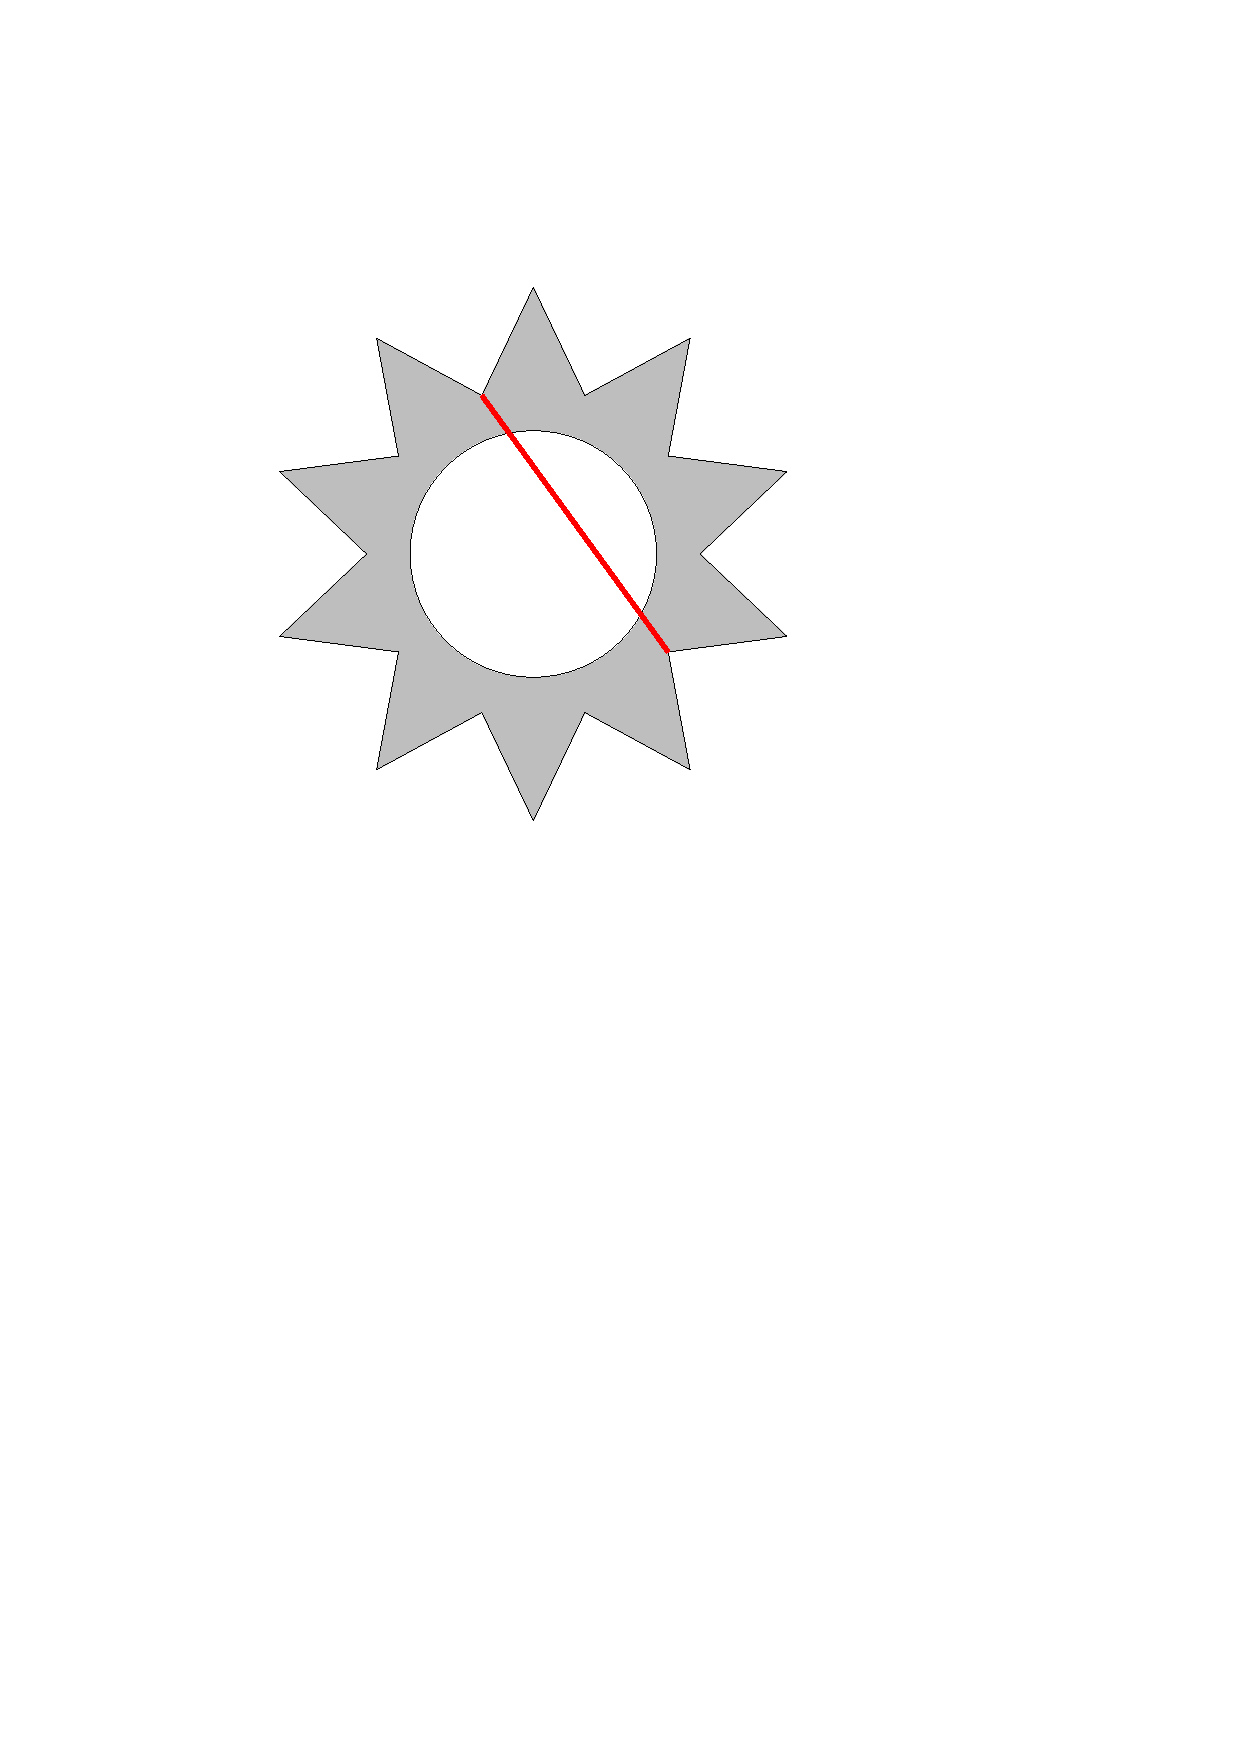
\includegraphics[width=3cm]{inefficient.pdf}}
            \hfill
            \onslide<1->{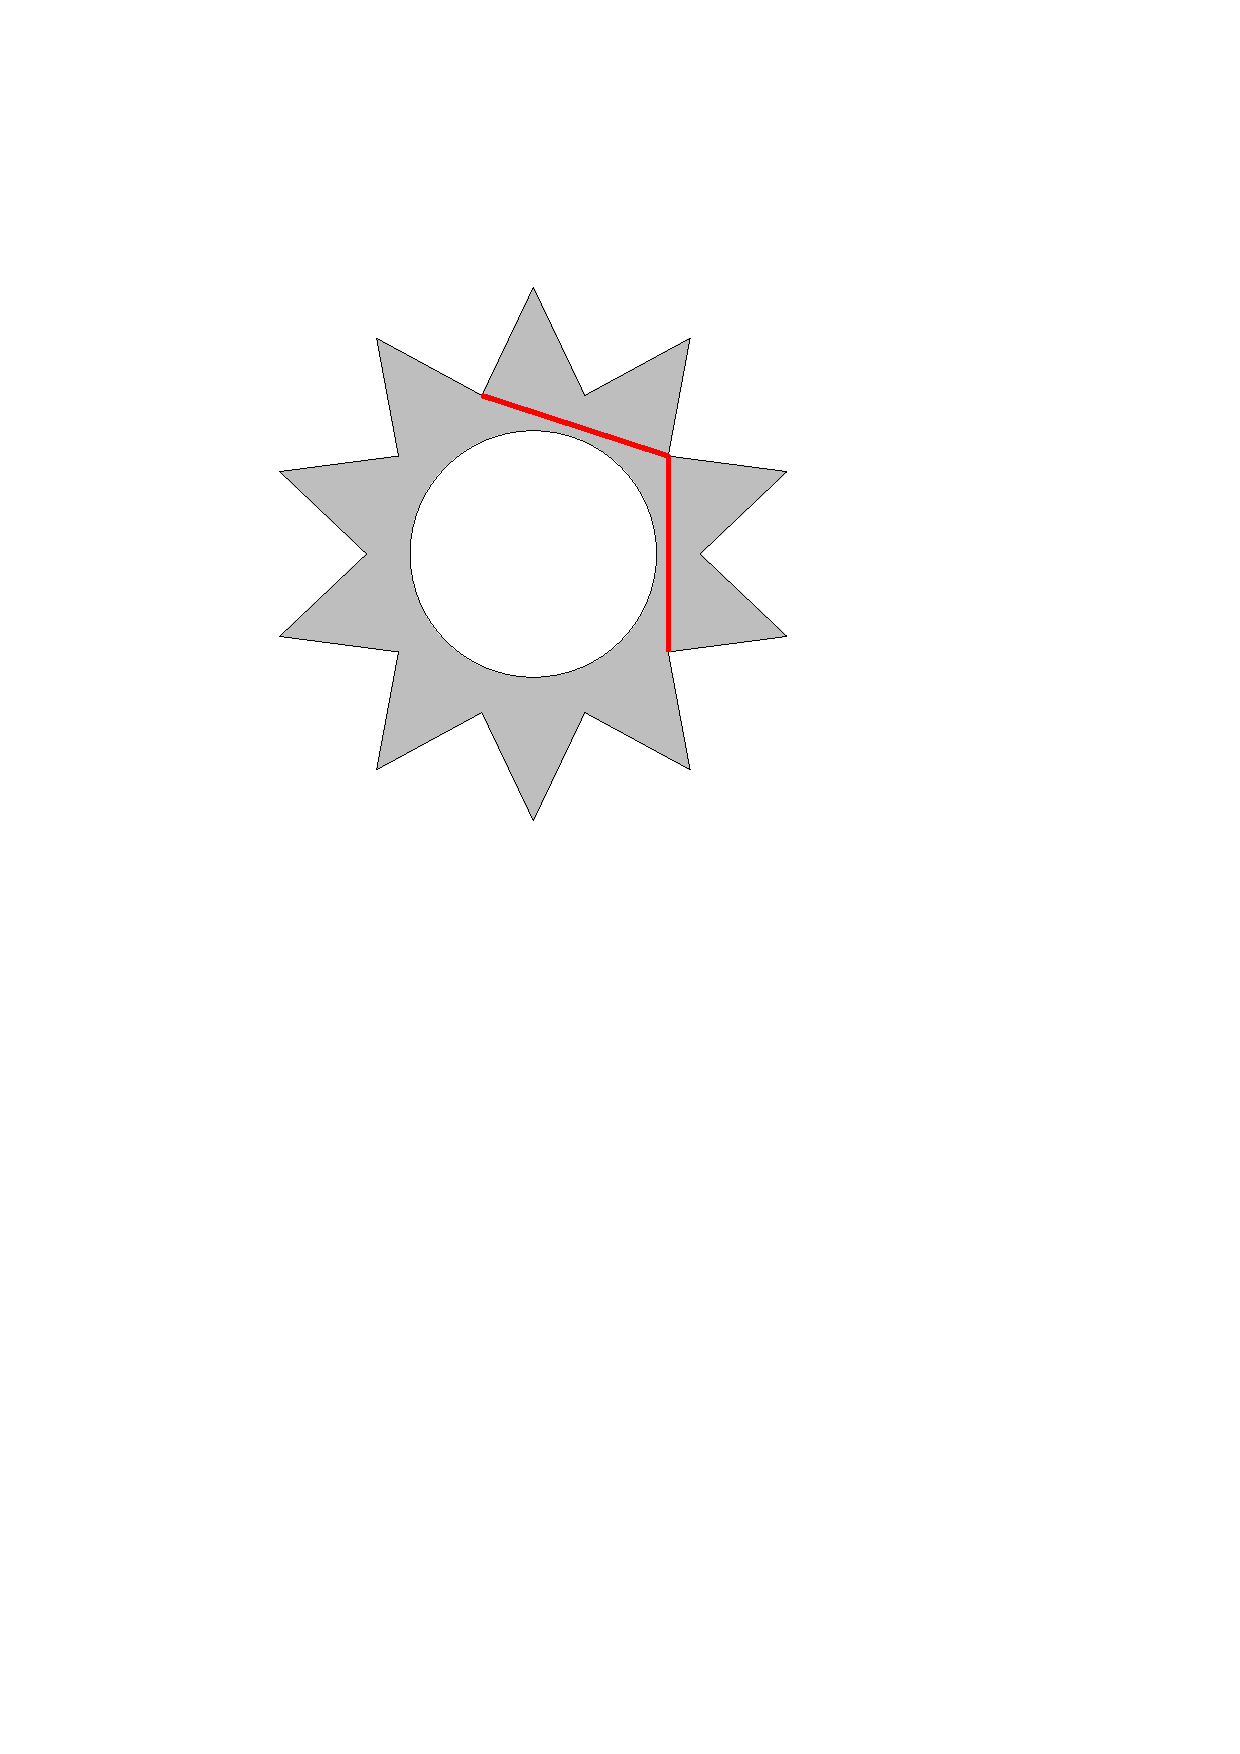
\includegraphics[width=3cm]{efficient.pdf}}
            \hfill
            \hfill% Silly LaTeX, requiring \hfill twice at the end of a line
\end{frame}

\begin{frame}
    \frametitle{\problemtitle}
    \begin{block}{Observation}
        Need to find $k$ coprime with $n$ which is as close to $\frac{n}{2}$ as possible.
    \end{block}
    \pause
    \begin{block}{Solution}
    	\begin{itemize}
    	\item Can use linear search, starting from $\frac{n}{2}$. \pause
    	\item Alternatively, use a direct formula:
    		\begin{itemize}
    		\item if $n \equiv 1 \mod 2$, take $k = \frac{n-1}{2}$,
    		\item if $n \equiv 2 \mod 4$, take $k = \frac{n}{2} - 2$,
    		\item if $n \equiv 0 \mod 4$, take $k = \frac{n}{2} - 1$.
    		\end{itemize}
    	\end{itemize}
    \end{block}
    \pause
    \solvestats
\end{frame}


%\begin{frame}
%    \frametitle{\problemtitle}
%    \begin{block}{Problem}
%        Use as much yarn as possible while building a dreamcatcher.\\
%        More formally, find integer $x$ between 1 and $\frac{n}{2}$ to maximize
%        $$\frac{lcm(n,x)}{x} \cdot 2\sin(\frac{x}{n}\pi).$$
%    \end{block}
%    \pause
%    \begin{block}{Observations}
%    \begin{itemize}
%        \item Trying all $x$ is too slow.
%        \pause
%        \item If $x$ is coprime to $n$, it maximizes the first term with $\frac{lcm(n,x)}{x} = n$.
%        \pause
%        \item The remaining part is monotone in $x$ and grows from 0 to 2.
%        \pause
%        \item So if we go with a coprime $x$, then the largest one is best.
%        \pause
%        \item This is actually optimal and can be found by going down from $\frac{n}{2}$.
%        \pause
%        \item We don't have to search for long. The largest prime gap in this range is 282.
%    \end{itemize}
%    \end{block}
%\end{frame}

%\begin{frame}
%    \frametitle{\problemtitle}
%    \begin{block}{Solution}
%        Find the largest number that is coprime to $n$ and smaller than $\frac{n}{2}$.
%    \end{block}
%    \pause
%    \begin{block}{Proof}
%    \begin{itemize}
%        \item Since there exists a prime between $\frac{n}{4}$ and $\frac{n}{2}$ (Bertrand's postulate), our solution is at least
%        $$n \cdot 2\sin(\pi/4) \approx 1.41n$$
%        \pause
%        \item If we choose any non-coprime $x$, then we have at most
%        $$\frac{n}{2} \cdot 2\sin(\pi/2) = n$$
%    \end{itemize}
%    \end{block}
%    \pause
%    \solvestats
%\end{frame}
